\subsection{Interfejs}
W drugiej iteracji poprawiony został wygląd strony przedstawiający listę produktów. Aktualnie najważniejszym aspektem charakteryzującym pojedynczą kolumnę w tabeli jest produkt, a nie jak w poprzedniej wersji złączenie produktu ze sklepem. W efekcie uzyskaliśmy efekt widoczny na poniższej grafice:

\begin{figure}[H]
\centering
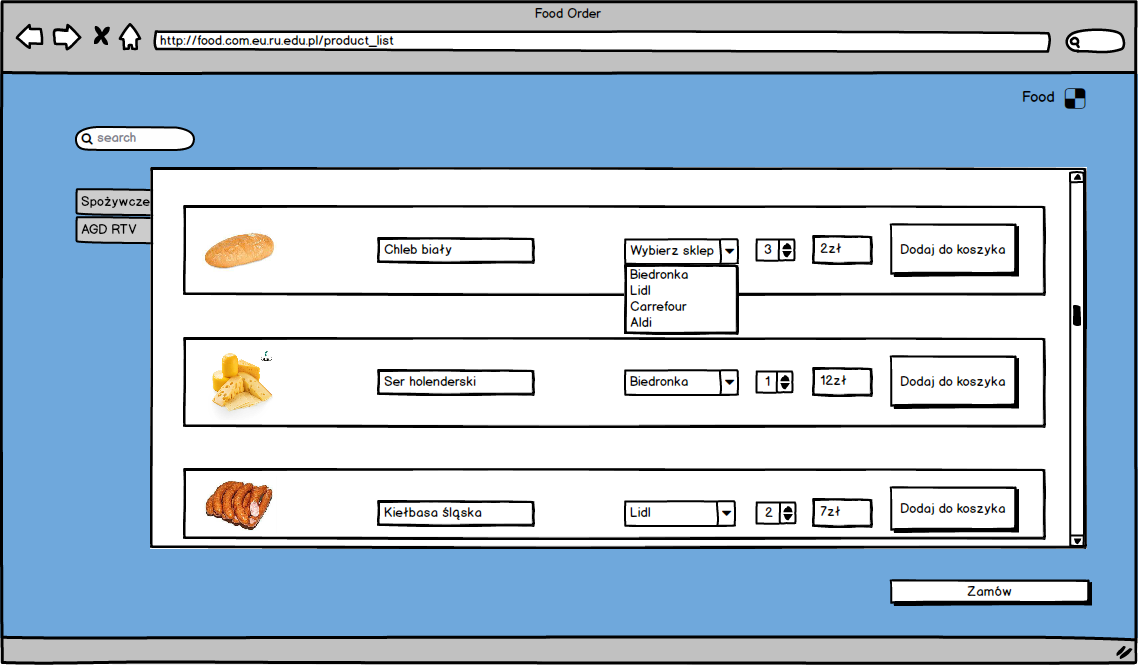
\includegraphics[width=15cm]{pictures/Lista_produktow_v2.png}
\caption{Druga iteracja wyboru produktu.}
\end{figure}

\begin{figure}[H]
\centering
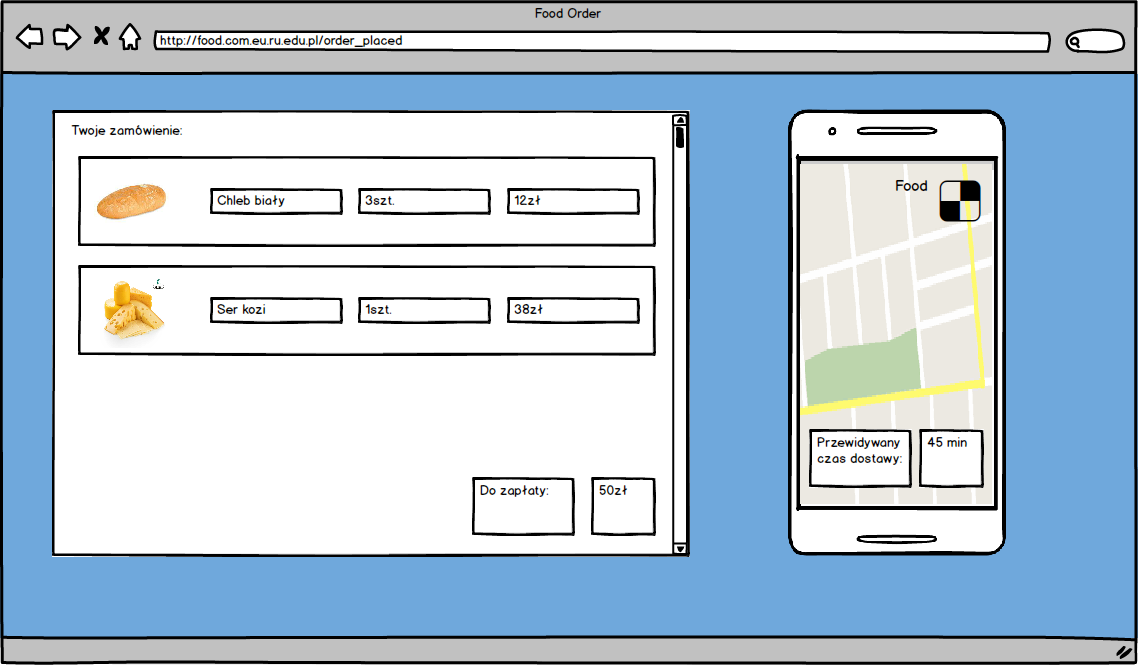
\includegraphics[width=15cm]{pictures/Zamowienie_zlozone_v2.png}
\caption{Druga iteracja ekranu złożonego zamówienia.}
\end{figure}

\subsection{Uwagi zamawiającego}
Klient zaakceptował widok w drugiej iteracji. Pragnął jednak, aby na każdym ekranie widoczny był taki sam \textit{header} z rozsuwanym menu, tzw. \textit{menu hamburger}.